\title{CS289 Initial Report: \\
Methods of handling missing data for classification
\vspace{15mm}}

\author{Rafael Valle\thanks{\href{mailto:rafaelvalle@berkeley.com}{\nolinkurl{rafaelvalle@berkeley.com}}.} \hspace{10mm}
Jason Poulos\thanks{\href{mailto:poulos@berkeley.edu}{\nolinkurl{poulos@berkeley.edu}}.}
\vspace{15mm}}

\date{\today}

%%%%%%%%%%%%%%%%%%%%%%%%%%%%%%%%%%%%%%%%%%%%%%%%%%
% Set document class
\documentclass[12pt]{article}

% Define packages
\usepackage{graphicx,amsfonts,psfrag,layout,subcaption,array,longtable,lscape,booktabs,dcolumn,natbib,amsmath,amssymb,amssymb,amsthm,setspace,epigraph,chronology,color, colortbl,caption,wasysym}
\usepackage[]{graphicx}\usepackage[]{color}
\usepackage[page]{appendix}
\usepackage{hyperref, url}
\usepackage[section]{placeins}
\usepackage[linewidth=1pt]{mdframed}
\usepackage[margin=1in]{geometry} %1 inch margins

% Footnotes stick at the bottom
\usepackage[bottom]{footmisc}

% New footnote characters
\usepackage{footmisc}
\DefineFNsymbols{mySymbols}{{\ensuremath\dagger}{\ensuremath\ddagger}\S\P
   *{**}{\ensuremath{\dagger\dagger}}{\ensuremath{\ddagger\ddagger}}}
\setfnsymbol{mySymbols}

% New tabular environment
\usepackage{tabularx}
\newcolumntype{Y}{>{\raggedleft\arraybackslash}X}% raggedleft column X

% Define appendix
\renewcommand*\appendixpagename{Appendix}
\renewcommand*\appendixtocname{Appendix}

% Position floats
\renewcommand{\textfraction}{0.05}
\renewcommand{\topfraction}{0.95}
\renewcommand{\bottomfraction}{0.95}
\renewcommand{\floatpagefraction}{0.35}
\setcounter{totalnumber}{5}

% Colors for highlighting tables
\definecolor{Gray}{gray}{0.9}

% Different font in captions
\newcommand{\captionfonts}{\scriptsize}

\makeatletter  % Allow the use of @ in command names
\long\def\@makecaption#1#2{%
  \vskip\abovecaptionskip
  \sbox\@tempboxa{{\captionfonts #1: #2}}%
  \ifdim \wd\@tempboxa >\hsize
    {\captionfonts #1: #2\par}
  \else
    \hbox to\hsize{\hfil\box\@tempboxa\hfil}%
  \fi
  \vskip\belowcaptionskip}
%\makeatother   % Cancel the effect of \makeatletter

% Set Spacing
%\doublespacing

%Theorem
\newtheorem{theorem}{Theorem}

% Number assumptions
\newtheorem*{assumption*}{\assumptionnumber}
\providecommand{\assumptionnumber}{}
\makeatletter
\newenvironment{assumption}[2]
 {%
  \renewcommand{\assumptionnumber}{Assumption #1}%
  \begin{assumption*}%
  \protected@edef\@currentlabel{#1}%
 }
 {%
  \end{assumption*}
 }
\makeatother

% Macros
\newcommand{\Adv}{{\mathbf{Adv}}}
\newcommand{\prp}{{\mathrm{prp}}}                  % How to define new commands
\newcommand{\calK}{{\cal K}}
\newcommand{\outputs}{{\Rightarrow}}
\newcommand{\getsr}{{\:\stackrel{{\scriptscriptstyle\hspace{0.2em}\$}}{\leftarrow}\:}}
\newcommand{\andthen}{{\::\;\;}}    %  \: \; for thinspace, medspace, thickspace
\newcommand{\Rand}[1]{{\mathrm{Rand}[{#1}]}}       % A command with one argument
\newcommand{\Perm}[1]{{\mathrm{Perm}[{#1}]}}
\newcommand{\Randd}[2]{{\mathrm{Rand}[{#1},{#2}]}} % and with two arguments
\newcommand{\E}{\mathrm{E}}
\newcommand{\ind}{\mathbb{I}} % Indicator function
\newcommand{\pr}{\mathbb{P}} % Generic probability
\newcommand{\ex}{\mathbb{E}} % Generic expectation
\newcommand{\Var}{\mathrm{Var}}
\newcommand{\Cov}{\mathrm{Cov}}
\newcommand{\cov}{\mathrm{Cov}}
\DeclareMathOperator*{\plim}{plim}
\newcommand\independent{\protect\mathpalette{\protect\independenT}{\perp}}
\def\independenT#1#2{\mathrel{\rlap{$#1#2$}\mkern2mu{#1#2}}}
\newcommand{\possessivecite}[1]{\citeauthor{#1}'s [\citeyear{#1}]}
\newcommand{\todo}[1]{{\color{red}{TO DO: \sc #1}}}

\begin{document}

\maketitle

\section{Motivation}
In our project, we plan to investigate techniques for handling missing data and
encoding categorical data such that it is appropriate to neural networks.  

% As a first step, we plan to use NNets for income prediction ($income \geq \$
% 50K/yr$) on the Adult dataset.

%Include necessary background information:
  % What is the application domain and/or field of research?
  % Why is the problem important?
  % What specific questions are you trying to answer?

Item nonresponse is a common problem in survey data in various domains. Several
techniques for data imputation (replace missing values with plausible ones) and
direct estimation (all missing data is analyzed using a maximum likelihood
approach) have been developed \cite{de2003prevention}.


In addition, given that categorical variables have no direct representation or computation scheme of the distance between its values, decision trees can be useful because they do not require distance metrics. However, they might not be suitable for problems where the decision boundary between classes is described by a second-order polynomial, for example.\cite{fayyad1996data}

\section{Data}
Our experimet will start with the Adult dataset and move to a larger sensus dataset.
\subsection{Adult data set}
\resizebox{\textwidth}{!}{
    \begin{tabular}{ l l | l l | l l}
      \hline
      Characteristics: & Multivariate &
      Observations: & 48842 &
      Area: & Social \\

      Features: & Categorical, Integer &
      Number of features: & 14 &
      Date Donated: & 1996-05-01 \\

      Associated Tasks: & Classification &
      Missing Values? & Yes &
      Number of Web Hits: & 559776 \\

      \hline
    \end{tabular}
}

\subsection{Benchmarks}
% Table comparing accuracies for different models

\subsection{Patterns of missing values}

\begin{figure}[htbp] 
   \centering
   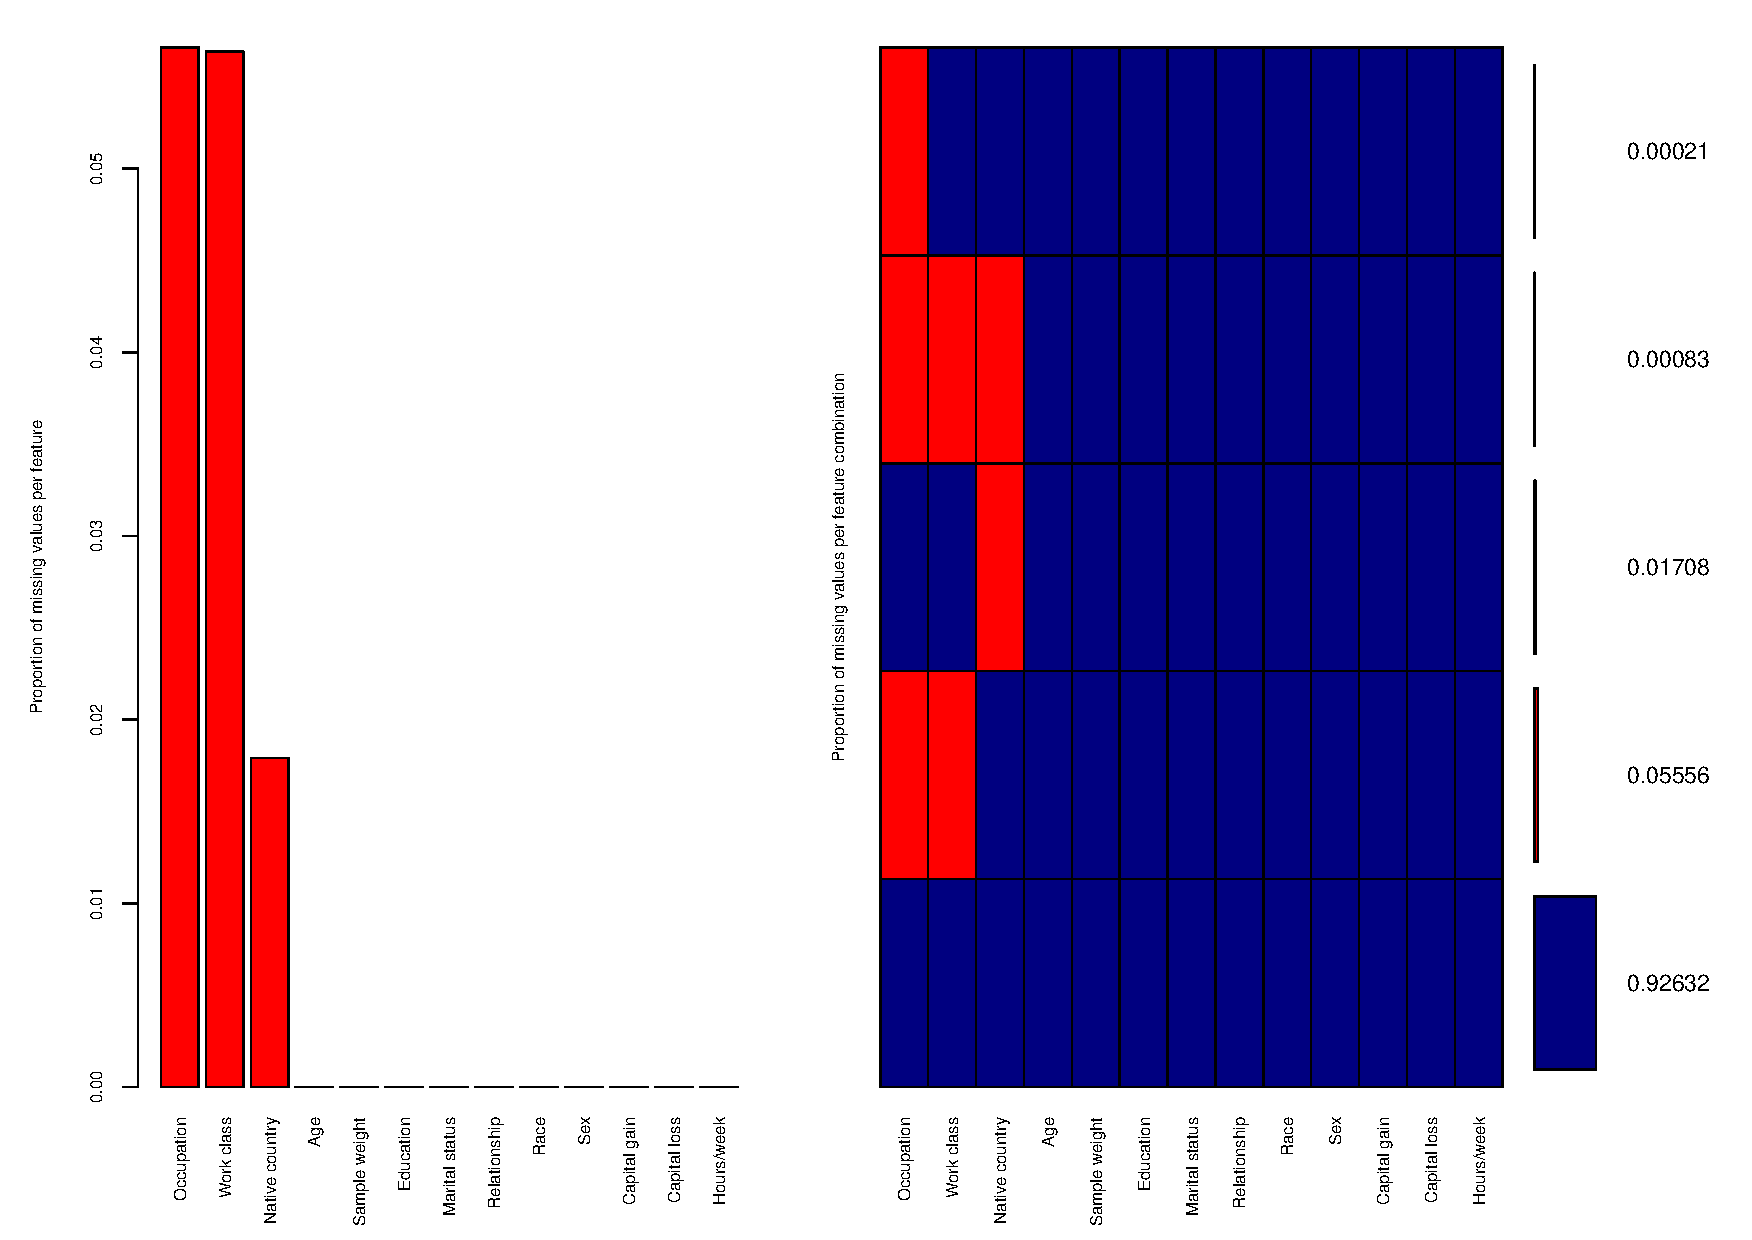
\includegraphics[scale=0.6]{proportion-missing.pdf} 
   \caption{Histogram of proportion of missing values in each feature (Left) and aggregation plot of all existing combinations of missing and non-missing values in the samples (Right).}
   \label{proportion-missing}
\end{figure}

\begin{figure}[htbp] 
   \centering
   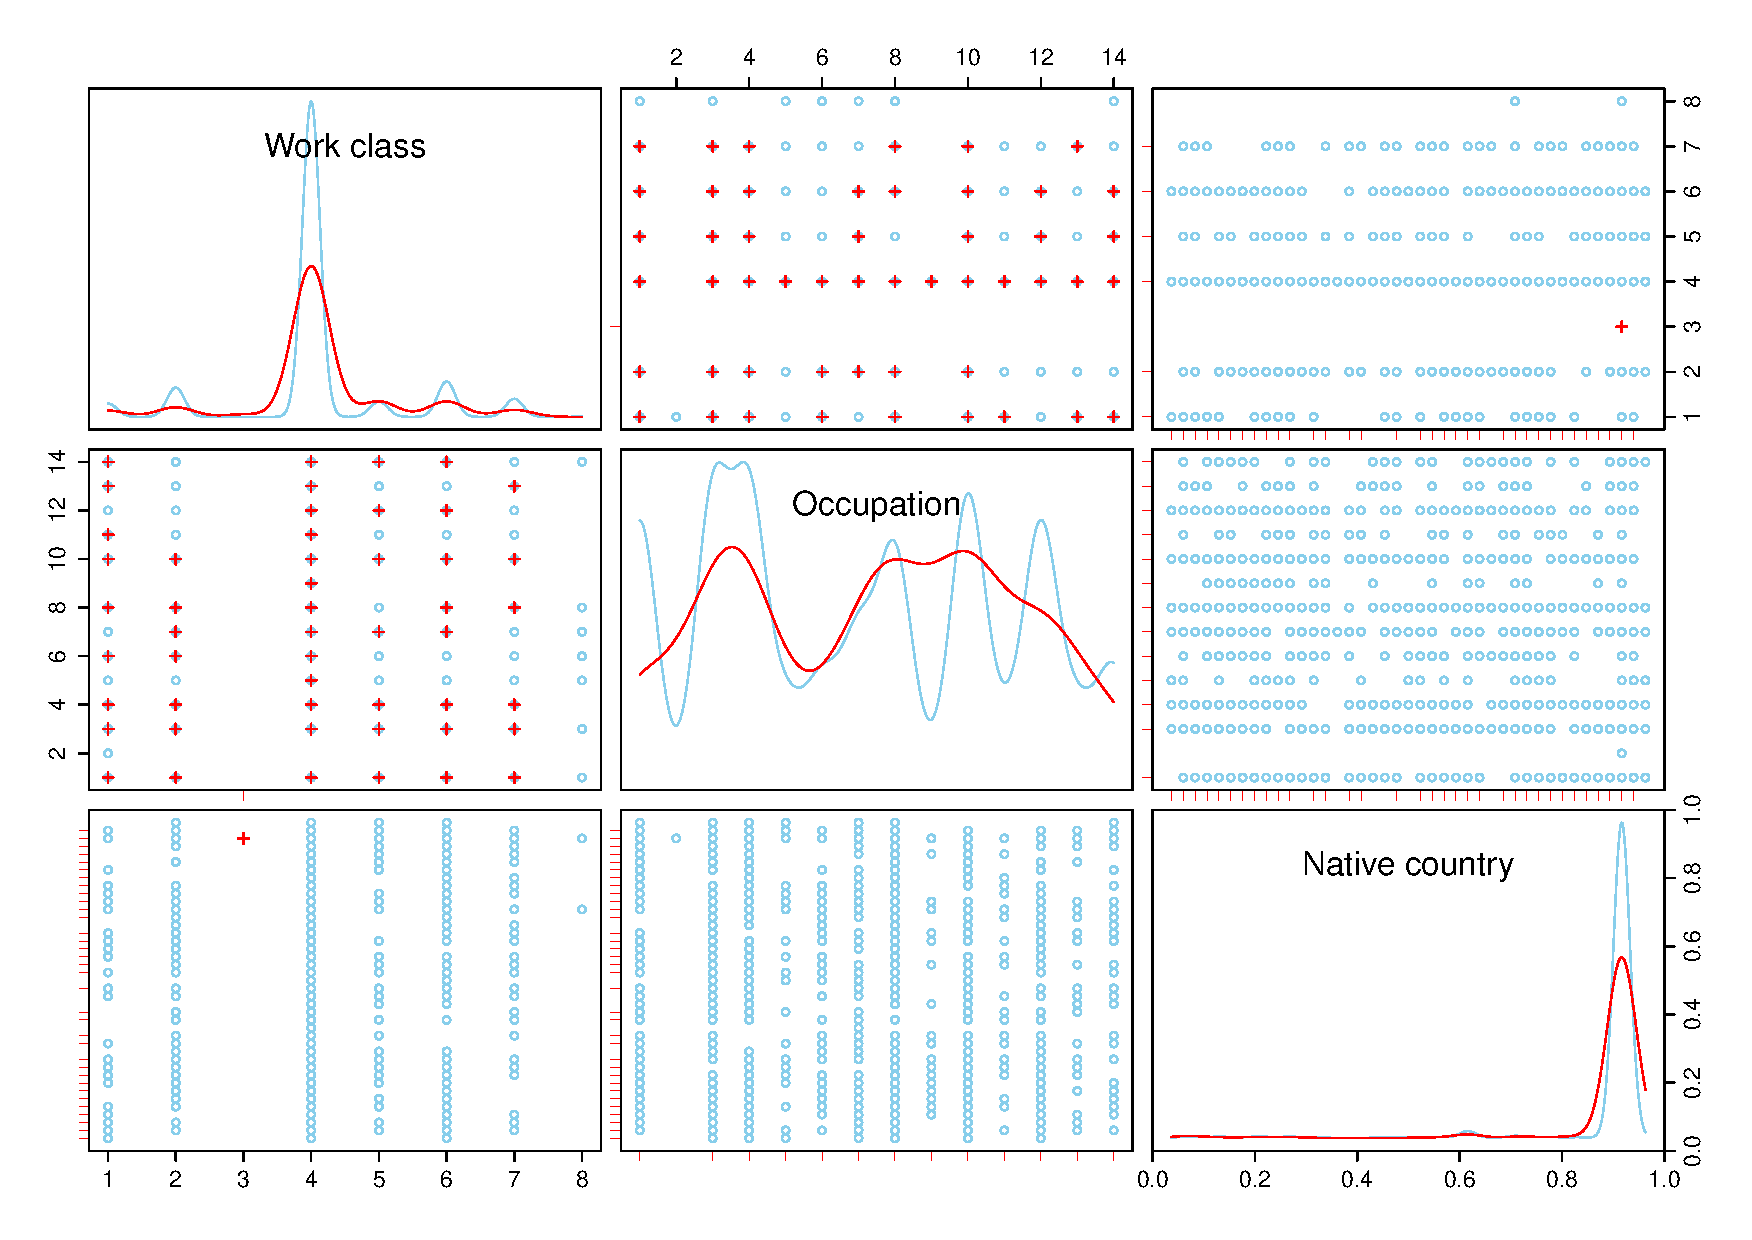
\includegraphics[scale=0.6]{scatter-matrix-missing.pdf} 
   \caption{Scatterplot Matrix of features with missing values. Blue represents observed values and red represents missing values.}
   \label{proportion-missing}
\end{figure}

% Table showing proportion of missing values for each feature

\section{Methods}

% Explain which methods you are planning to use and why.

\subsection{Techniques for handling missing data}
We divide imputation methods into six groups listed
below\cite{batista2003analysis}. Assuming that these techniques are easy to
implement, we would like to compare their efficiency in imputing the missing
values.

\begin{enumerate}
\item Case substitution: one observation with missing data is replaced with
    another non-sampled instance.
\item Mean or mode imputation: Replace the missing data with the mean or median of
    the feature vector. This is the most naive approach and since the missing
    variables in the ADULT dataset are all categorical, using the mean is not
    appropriated.
\item One-hot: Create an binary variable to indicate whether or not a specific
    feature is missing. This technique was mentioned by Isabelle
\item Hot deck and cold deck: Compute the K-Nearest Neighbors of the
    observation with missing data and assign the mean or median of the K-neighbors
    to the missing data. A similar technique is used in Airbnb's fraud detection
    algorithm.
\item Prediction Model: train a prediction model, e.g. logistic regression and
    baggin, with all features except the feature with the missing variable to
    predict the missing value. This requires correlation amongst variables to
    exist.
\item Factor analysis: Perform some sort of factorization on the design
    matrix, project the design matrix onto the first two eigen vectors and
    replace the missing values by the values that might be given by the
    projected design matrix.
\end{enumerate}

\subsection{Neural networks for classification with categorical and
quantitative features}  Techniques for handling categorical data in neuronal
networks include encoding the categorical values into numeric values, using
binary encoding. These methods, however, have many drawbacks including
unnecessarily increasing the dimensionality or not preserving the similarity
information embedded betweeng categorical values\cite{hsu2006generalizing}.

More elaborate techniques include information theoretic measures
\cite{wang2008categorical}, training separate output units for
each of the allowed combination of values of the categorical independent
variables\cite{brouwer2002feed}, and using distance
hierarchies\cite{hsu2006generalizing}.
\section{Anticipated results}

\pagebreak

%Bibliography
\bibliographystyle{plainnat}
\bibliography{refs}

%%Appendix
%\pagebreak
%\begin{appendices}
%
%\begin{figure}[htbp]
%\begin{center}
%\includegraphics[width = 1\textwidth]{rmse_ratec_rates}
%\caption{Simulated RMSE, binned by compliance rate and percent eligible for the RCT. Darker tiles correspond to worse estimates of PATT.}
%\label{fig:sim_tiles}
%\end{center}
%\end{figure}
%
%\end{appendices}

\itemize
\end{document}


